\documentclass[../../main.tex]{subfiles}
\graphicspath{{../../image/}{../../figure/}}
\begin{document}

\section{连续介质物理中的平衡律}\label{section:ch02-平衡律}

考察一个具有参考构型 $\mathscr{B}\subset\mathbb{R}^{m}$ 的物体在时间区间 $(t_{1},t_{2})$ 上的运动 $\chi$。连续介质物理的典型平衡律假定：物体任一部分中所储存的某一广延量在任一时间段内的变化，由该时间段内通过边界的通量与内部的产生量所平衡。将空间与时间融合为时空后，上述陈述给出\cref{chapter:ch01-平衡律}中所考虑的那类平衡律，最终归结为该章一般形式的场方程。


为将\cref{chapter:ch01-平衡律}的记号适配到当前情形，我们取时空 $\mathbb{R}^{m+1}$ 作为 ambient 空间 $\mathbb{R}^{k}$，并令 $\mathscr{X}=\mathscr{B}\times(t_{1},t_{2})$，$X=(x,t)$。参照\cref{chapter:ch01-平衡律}中的平衡律一般形式，我们将通量密度场 $A$ 分解为一个 $n\times m$ 矩阵值空间部分 $\Psi$ 与一个 $\mathbb{R}^{n}$ 值时间部分 $\Theta$，即 $A=[-\Psi\mid\Theta]$。在上一节引入的记号下，该平衡律现取形式
\begin{align}
\dot{\Theta}=\mathrm{Div}\,\Psi+P.
\label{align:ch02-2-2-1}
\end{align}
这就是连续介质物理典型平衡律的参考场方程。场 $\Theta$ 是被平衡量的密度；$\Psi$ 是通过物质曲面的通量密度场；$P$ 是产生密度。


相应的空间场方程可借助\cref{chapter:ch01-平衡律}导出。将 $(x,t)$ 映到 $(\chi(x,t),t)$ 的映射 $X^{*}$ 是 $\mathscr{X}$ 到 $\mathbb{R}^{m+1}$ 中某子集 $\mathscr{X}^{*}$ 的双 Lipschitz 同胚，其 Jacobi 矩阵为（参见前述一般变换公式、\eqref{align:ch02-2-1-1} 与 \eqref{align:ch02-2-1-2}）：

\begin{align}
J=\begin{bmatrix}F\vline v\\ 0\vline 1\end{bmatrix}.
\label{align:ch02-2-2-2}
\end{align}

注意前述相容性条件由\eqref{align:ch02-2-1-3}成立。\cref{chapter:ch01-平衡律}中相应定理与注记现在蕴涵：若 $\Theta\in L^{1}_{\mathrm{loc}}(\mathscr{X};\mathbb{R}^{n})$，$\Psi\in L^{1}_{\mathrm{loc}}(\mathscr{X};\mathbb{M}^{n\times k})$，$P\in L^{1}_{\mathrm{loc}}(\mathscr{X};\mathbb{R}^{n})$，则\eqref{align:ch02-2-2-1} 在 $\mathscr{X}$ 上按分布意义成立，当且仅当

\begin{align}
\Theta^{*}_{t}+\mathrm{div}\,(\Theta^{*}v^{\top})=\mathrm{div}\,\Psi^{*}+P^{*}
\label{align:ch02-2-2-3}
\end{align}
在 $\mathscr{X}^{*}$ 上按分布意义成立，其中场 $\Theta^{*}\in L^{1}_{\mathrm{loc}}(\mathscr{X}^{*};\mathbb{R}^{n})$、$\Psi^{*}\in L^{1}_{\mathrm{loc}}(\mathscr{X}^{*};\mathbb{M}^{n\times m})$、$P^{*}\in L^{1}_{\mathrm{loc}}(\mathscr{X}^{*};\mathbb{R}^{n})$ 由下式定义：
\begin{align}
\Theta^{*}=(\det F)^{-1}\Theta,\qquad\Psi^{*}=(\det F)^{-1}\Psi F^{\top},\qquad P^{*}=(\det F)^{-1}P.
\label{align:ch02-2-2-4}
\end{align}

于是已经确立：连续介质物理平衡律的参考（Lagrange）场方程\eqref{align:ch02-2-2-1}与空间（Euler）场方程\eqref{align:ch02-2-2-3}通过\eqref{align:ch02-2-2-4}相联系，并且在本文所考虑的场函数类中是等价的。

如我们所见，为从 Lagrange 坐标过渡到 Euler 坐标（或反之），必须对一个并非预先给定、而是由运动本身生成的双 Lipschitz 同胚应用\cref{chapter:ch01-平衡律}，而该运动同时也影响被平衡的场。这种耦合与参考和空间平衡律是否等价无关，但却无端给这个问题蒙上了一层神秘色彩。


为预告即将讨论的材料对称性，有必要考察场 $\Theta,\Psi,P$ 与 $\Theta^{*},\Psi^{*},P^{*}$ 在物体参考构型的\emph{等容}变化下如何变换；这种变化由一个将 $\mathscr{B}$ 双 Lipschitz 同胚到另一参考空间 $\mathbb{R}^{m}$ 中某子集 $\bar{\mathscr{B}}$ 的映射 $\bar{x}$ 诱导，其 Jacobi 矩阵为
\begin{align}
H=\frac{\partial\bar{x}}{\partial x},\qquad\det H=1,
\label{align:ch02-2-2-5}
\end{align}
见\cref{figure:ch02-等容变换示意图}。

\begin{figure}[ht]
\centering
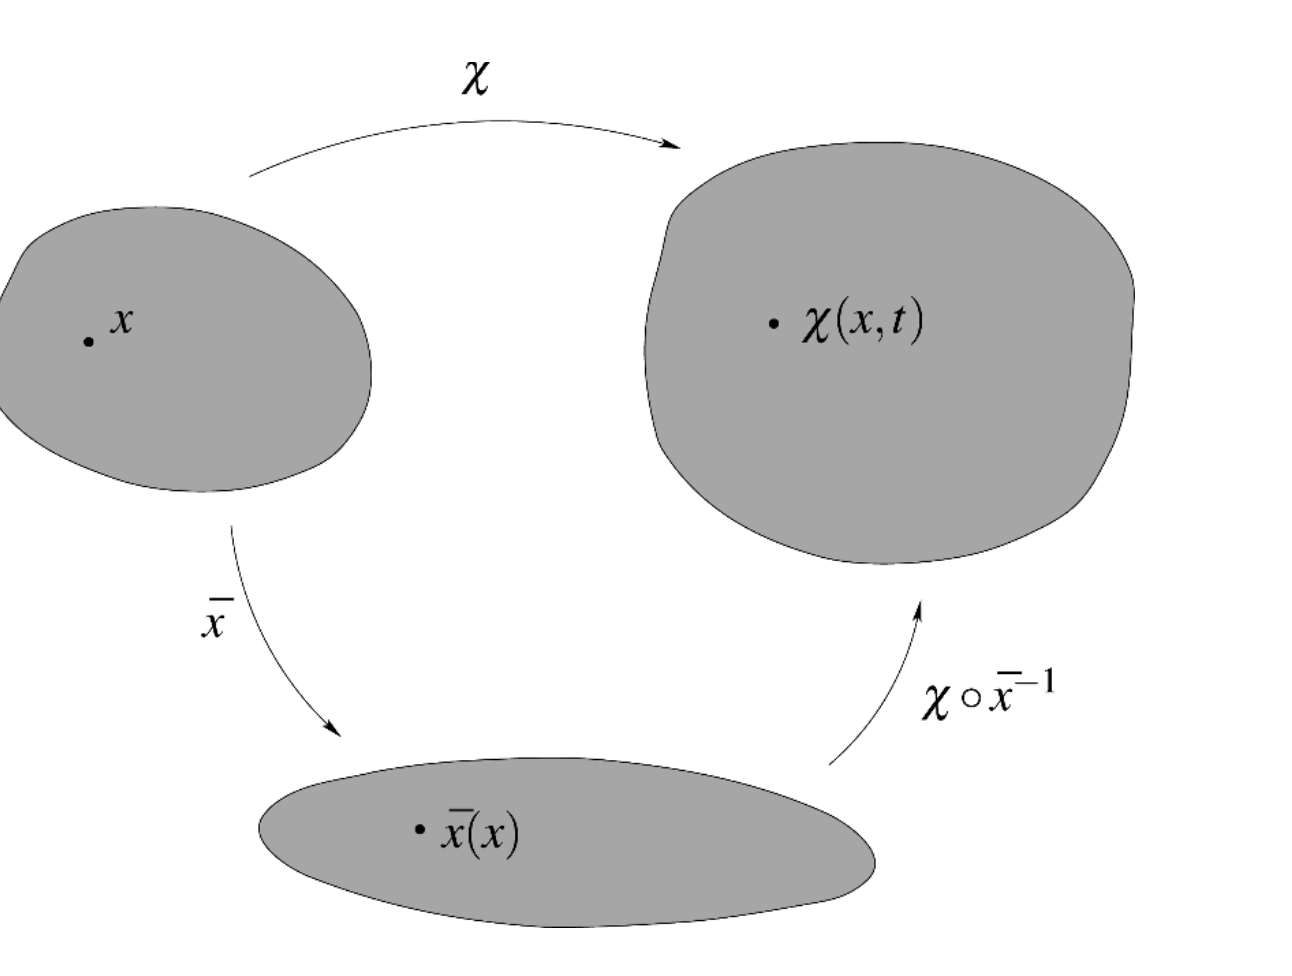
\includegraphics[width=0.7\textwidth]{ch02-fig02-01.png}
\caption{参考构型的等容变化：由映射 $\bar{x}:\mathscr{B}\to\bar{\mathscr{B}}$ 诱导，复合运动为 $\chi\circ\bar{x}^{-1}$。}
\label{figure:ch02-等容变换示意图}
\end{figure}

由\cref{chapter:ch01-平衡律}，$\mathscr{B}$ 上的 Lagrange 场方程\eqref{align:ch02-2-2-1} 将变换为 $\bar{\mathscr{B}}$ 上形式完全相同的方程，场 $\bar{\Theta},\bar{\Psi},\bar{P}$ 与 $\Theta,\Psi,P$ 之间由下式联系：

\begin{align}
\bar{\Theta}=\Theta,\qquad\bar{\Psi}=\Psi H^{\top},\qquad\bar{P}=P.
\label{align:ch02-2-2-6}
\end{align}

在相应的 Euler 场方程中，场 $\bar{\Theta}^{*},\bar{\Psi}^{*},\bar{P}^{*}$ 通过\eqref{align:ch02-2-2-4}得到：$\bar{\Theta}^{*}=(\det\bar{F})^{-1}\bar{\Theta}$，$\bar{\Psi}^{*}=(\det\bar{F})^{-1}\bar{\Psi}\bar{F}^{\top}$，$\bar{P}^{*}=(\det\bar{F})^{-1}\bar{P}$，其中 $\bar{F}$ 表示相对于新参考构型 $\bar{\mathscr{B}}$ 的变形梯度。由链式法则，$\bar{F}=FH^{-1}$，于是
\begin{align}
\bar{\Theta}^{*}=\Theta^{*},\qquad\bar{\Psi}^{*}=\Psi^{*},\qquad\bar{P}^{*}=P^{*},
\label{align:ch02-2-2-7}
\end{align}
即，正如所预期的，空间场不受改变物体参考构型的影响。

在连续介质物理中，理论由其适用的平衡律清单来标识。下一节将给出热力学连续介质力学这一说明性例子。但应当注意，除具有物理内容的平衡律之外，还有一些平衡律仅仅表达有用的、纯运动学的性质。方程\eqref{align:ch02-2-1-8}（即 $\dot{F}=\nabla v$）表达场 $F$ 与 $v$ 之间的协调性，就是这方面的一个例子。

初读时，可跳过本节余下内容（它处理一个留待将来使用的特殊专题），直接进入下一节\cref{section:ch02-连续介质热力学平衡律}。

下面我们对 $m=3$ 推导一组运动学平衡律，其参考形式相当复杂，而空间形式非常简单甚至平凡。这将展示在 Lagrange 与 Euler 表述之间切换的用处。

\begin{definition}[零 Lagrange 量]\label{definition:ch02-零Lagrange量}
设 $\varphi$ 是定义在集合 $\{F\in\mathbb{M}^{3\times 3}:\det F>0\}$ 上的光滑函数。若与泛函 $\int\varphi(F)\,\mathrm{d}x$ 相关联的 Euler--Lagrange 方程
\begin{align}
\mathrm{Div}\,[\partial_{F}\varphi(F)]=0
\label{align:ch02-2-2-8}
\end{align}
对每个光滑变形梯度场 $F$ 都成立，则称 $\varphi$ 为一个\emph{零 Lagrange 量}。
\end{definition}

任何零 Lagrange 量 $\varphi$ 都可表示为 $F$、其行列式 $\det F$ 及其伴随矩阵 $F^{*}=(\det F)F^{-1}=(\partial_{F}\det F)^{\top}$ 的仿射函数：
\begin{align}
\varphi(F)=\mathrm{tr}(AF)+\mathrm{tr}(BF^{*})+\alpha\det F+\beta.
\label{align:ch02-2-2-9}
\end{align}

将\eqref{align:ch02-2-2-8}与 $\dot{F}=\nabla v$ 相结合，可以推出：若 $\varphi$ 是任一形如\eqref{align:ch02-2-2-9}的零 Lagrange 量，则对任何具有变形梯度 $F$ 和速度 $v$ 的光滑运动，守恒律
\begin{align}
\dot{\varphi}(F)=\mathrm{Div}\,[v^{\top}\partial_{F}\varphi(F)]
\label{align:ch02-2-2-10}
\end{align}
成立。

此处的目的是证明：对任一零 Lagrange 量\eqref{align:ch02-2-2-9}，“准静态”守恒律\eqref{align:ch02-2-2-8}以及“运动学”守恒律\eqref{align:ch02-2-2-10}实际上对仅仅 Lipschitz 连续的运动也成立，即
\begin{align}
\mathrm{Div}\,(\partial_{F}F)=0,
\label{align:ch02-2-2-11}
\end{align}
\begin{align}
\mathrm{Div}\,(\partial_{F}F^{*})=0,
\label{align:ch02-2-2-12}
\end{align}
\begin{align}
\mathrm{Div}\,(\partial_{F}\det F)=0,
\label{align:ch02-2-2-13}
\end{align}
\begin{align}
\dot{F}=\mathrm{Div}\,(v^{\top}\partial_{F}F),
\label{align:ch02-2-2-14}
\end{align}
\begin{align}
\dot{F}^{*}=\mathrm{Div}\,(v^{\top}\partial_{F}F^{*}),
\label{align:ch02-2-2-15}
\end{align}
\begin{align}
\dot{\det F}=\mathrm{Div}\,(v^{\top}\partial_{F}\det F),
\label{align:ch02-2-2-16}
\end{align}
对任一有界可测变形梯度场 $F$ 和速度场 $v$ 成立。

显然，\eqref{align:ch02-2-2-11} 是平凡的，而\eqref{align:ch02-2-2-14} 不过是熟悉的 $\dot{F}=\nabla v$ 的另一种写法。此外，由于
\begin{align}
\frac{\partial F^{*}_{\alpha i}}{\partial F_{j\beta}}=\sum_{k=1}^{3}\sum_{\gamma=1}^{3}\varepsilon_{ijk}\varepsilon_{\alpha\beta\gamma}F_{k\gamma},
\label{align:ch02-2-2-17}
\end{align}
其中 $\varepsilon_{ijk}$ 和 $\varepsilon_{\alpha\beta\gamma}$ 是标准置换符号，而 $\partial F_{k\gamma}/\partial x_{\beta}=\partial^{2}\chi_{k}/\partial x_{\beta}\partial x_{\gamma}$ 关于 $(\beta,\gamma)$ 对称，$\varepsilon_{\alpha\beta\gamma}$ 关于 $(\beta,\gamma)$ 反对称，由此即得\eqref{align:ch02-2-2-12}。

为看出\eqref{align:ch02-2-2-13}，考虑平凡平衡律\eqref{align:ch02-2-2-3}，取 $\Theta^{*}=0$，$\Psi^{*}=I$，$P^{*}=0$，写出其 Lagrange 形式\eqref{align:ch02-2-2-1}，其中由\eqref{align:ch02-2-2-4}，$\Theta=0$，$\Psi=(\det F)(F^{\top})^{-1}=(F^{*})^{\top}=\partial\det F/\partial F$，$P=0$。类似地，\eqref{align:ch02-2-2-16} 是平凡平衡律\eqref{align:ch02-2-2-3} 在取 $\Theta^{*}=1$，$\Psi^{*}=v^{\top}$，$P^{*}=0$ 时的 Lagrange 形式\eqref{align:ch02-2-2-1}。事实上，在该情形下，由\eqref{align:ch02-2-2-4} 推得 $\Theta=\det F$，$\Psi=(\det F)(F^{-1}v)^{\top}=(F^{*}v)^{\top}=v^{\top}(\partial\det F/\partial F)$，$P=0$。

还需验证\eqref{align:ch02-2-2-15}。我们从 Euler 坐标中的简单守恒律
\begin{align}
(F^{-1})_{t}=(\mathrm{d}x)_{t}=\mathrm{d}x_{t}=-\mathrm{d}(F^{-1}v)
\label{align:ch02-2-2-18}
\end{align}
出发，通过\eqref{align:ch02-2-2-4}导出其 Lagrange 形式\eqref{align:ch02-2-2-1}。于是 $\Theta=(\det F)F^{-1}=F^{*}$，而通量 $\Psi$ 的分量形式为
\begin{align}
\Psi_{\alpha i\beta}=\sum_{j=1}^{3}(\det F)\bigl[F^{-1}_{\beta j}F^{-1}_{\alpha i}-F^{-1}_{\alpha j}F^{-1}_{\beta i}\bigr]v_{j}.
\label{align:ch02-2-2-19}
\end{align}
方括号中的量在 $\alpha=\beta$ 和/或 $i=j$ 时为零；否则它表示矩阵 $F^{-1}$ 的一个子式，因而等于 $\det F^{-1}$ 乘以矩阵 $(F^{-1})^{-1}=F$ 的相应元素。于是，回顾\eqref{align:ch02-2-2-17}，
\begin{align}
(\det F)\bigl[F^{-1}_{\beta j}F^{-1}_{\alpha i}-F^{-1}_{\alpha j}F^{-1}_{\beta i}\bigr]=\sum_{k=1}^{3}\sum_{\gamma=1}^{3}\varepsilon_{ijk}\varepsilon_{\alpha\beta\gamma}F_{k\gamma}=\frac{\partial F^{*}_{\alpha i}}{\partial F_{j\beta}},
\label{align:ch02-2-2-20}
\end{align}
这就证明了\eqref{align:ch02-2-2-15}。

\end{document}
